\section{Introduction}
\label{sec:Introduction}

The discovery of a neutral boson with a measured mass of around 125 GeV at the Large Hadron Collider (LHC) in 2012 \cite{HIGG-2012-27, CMS-HIG-12-028, HIGG-2014-14} opens the question of whether this is the Higgs boson of the Standard Model (SM) or part of an extended scalar sector. Indeed, charged Higgs bosons \footnote{Charge-conjugate is implied elsewhere in this note.} are predicted in several extensions of the SM, which add a second doublet \cite{T.D.Lee-1973, G.Branco-2012, K.Inoue-1982, T.Cheng-1989} or triplets \cite{T.Cheng-1989, J.Schechter-1980, G.Lazarides-1981, R.N.Mohapatra-1981, M.Magg-1980} to its scalar sector. In CP-conserving Two-Higgs-Doublet Models (2HDMs) $H^{+}$ production and decay at tree level depend on its mass and two parameters: the mixing angle $\alpha$ of the neutral CP-even Higgs bosons, and the ratio of the vacuum expectation values of the two Higgs doublets ($\tan{\beta}$).

\begin{figure}[H]
  \centering
  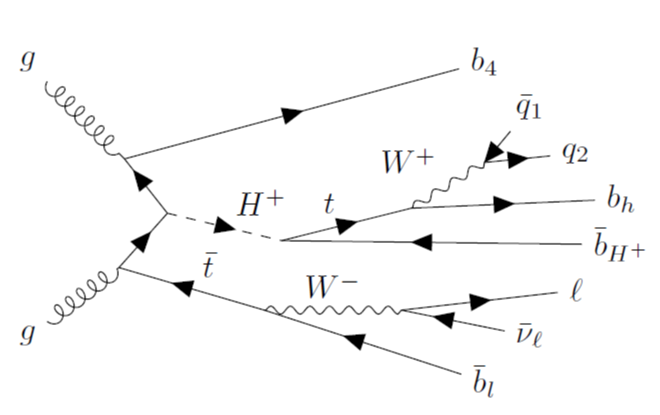
\includegraphics[keepaspectratio,scale=0.5]{images/Introduction/FeynmanDiagram_Htb.png}
  \caption{Feynman diagram for $pp{\rightarrow}tbH^{+}{\rightarrow}tb(tb)$}
  \label{fig:FeynmanDiagram_Htb}
\end{figure}


\vskip.2\baselineskip

For $H^{+}$ masses above the top-quark mass the leading production mode is $gg{\rightarrow}tbH^{+}$ and, close to the alignment limit when $\cos{({\beta}-{\alpha})}{\approx}0$, the dominant decay mode is $H^{+}{\rightarrow}tb$. For lower $H^{+}$ masses, the dominant decay mode is $H^{+}{\rightarrow}{\tau}{\nu}$, as well as for large values of $\tan{\beta}$ irrespective of the charged Higgs mass. Therefore, the two decay modes naturally complement each other in searches for charged Higgs bosons.

\vskip.2\baselineskip

The ATLAS and CMS collaborations have searched for charged Higgs bosons in $pp$ collisions at $\sqrt{s}=7,8$ and 13 TeV, probing the mass range below the top-quark mass in the $\tau\nu$ \cite{HIGG-2012-09, HIGG-2012-22, HIGG-2013-30, CMS-HIG-11-019, CMS-HIG-14-023, HIGG-2016-11}, $cs$ \cite{HIGG-2012-10, CMS-HIG-13-035}, and $cb$ \cite{CMS-HIG-16-030} decay modes, as well as above the top-quark mass in the $\tau\nu$ and $tb$ decay modes \cite{HIGG-2013-30, CMS-HIG-14-023, HIGG-2016-11, HIGG-2013-28, HIGG-2015-11, HIGG-2017-04, HDBS-2021-02, CMS-HIG-18-004, CMS-HIG-18-015, EXOT-2018-32}. In addition, $H^{+}{\rightarrow}WZ$ was searched for in the vector-boson-fusion production mode \cite{HIGG-2014-13, CMS-HIG-16-027}. No evidence for charged Higgs bosons was found in any of these searches.

\vskip.2\baselineskip

This note presents a search for $H^{+}$ production in the $H^{+}{\rightarrow}tb$ decay mode using $pp$ collisions at $\sqrt{s}=13$ TeV. Events with one charged lepton ($l=e,\mu$) and jets in the final state are considered. Compared with the previous analysis using the same final state and the dataset \cite{HDBS-2021-02} (so-called `resolved analysis), boosted top tagging technique is used to identify a hadronically decaying top quark originated from the decay of the heavy $H^{+}$. This technique allows to improve sensitivities in the high mass regions, where all top decay products are merged into a single large-R jet, and, therefore, cannot be reconstructed in the resolved analysis \cite{HDBS-2021-02}. 
%Exclusive regions are defined according to the number of jets tagged as originating from the hadronisation of a top quark and $b$-quark.
To separate the signal from the SM background, multivariate discriminants are employed in the regions where the signal rate is expected to be the largest. Limits on the $H^{+}{\rightarrow}tb$ production cross-section are set by a simultaneous fit of BDT distributions.

\vskip.2\baselineskip

Furthermore, the analysis technique is extended to a search for the $W'{\rightarrow}tb$ decay, where $W'$ is produced in association with $tb$. Several theories beyond the SM predict heavy-charged gauge bosons, which are usually referred to as $W'$ bosons\cite{dienes1999grand,weinberg1979implications,susskind1979dynamics,dimopoulos1979mass,eichten1980dynamical,muller1996topflavor}. Such $W'$ bosons can be heavy enough to decay into a top quark and a bottom quark. Some models predict $W'$ bosons that preferably couple to quarks or third-generation fermions \cite{burdman2006resonances,malkawi1996model,pati1974lepton,hill1995topcolor}. Unlike the $W$ boson, which only couples to left-handed fermions, the chirality of the interaction of the $W'$ boson can be left or right-handed, or a mixture of the two. In models where the right-handed neutrinos are heavier than the right-handed $W'$ boson, such $W'$ bosons cannot be searched for in the leptonic decay modes. We search for $W'$ bosons produced in association with a top quark and a bottom quark: Figure \ref{fig:FeynmanDiagram_Htb} illustrates this production process if we replace $H^{+}$ with $W'$. 
%as illustrated in Figure \ref{fig:FeynmanDiagram_Htb}, in which $H^{+}$ is replaced to $W'$.


Formerly, $W'$ bosons decaying into a top quark and a bottom quark were searched for in collisions between a quark and an antiquark of any flavour, where the $W'$ boson is singly produced without a top quark.  D0 \cite{abazov2011search} and CDF \cite{aaltonen2009search} Collaborations at the Tevatron and CMS \cite{CMS-EXO-12-001,CMS-B2G-12-010,CMS-B2G-17-010,CMS-B2G-20-005} and ATLAS \cite{TOPQ-2012-19,EXOT-2013-14,EXOT-2017-02,EXOT-2016-18} experiments at the LHC have published such search results.


The analysis replies on ATLAS official background as well as requested $H^+$ and $W'$ signal samples, as detailed in Section~\ref{sec:DataAndMC}, with the TOPQ1 derivation. The ntuples are produced using the TTHbbAnalysis software package.\footnote{https://gitlab.cern.ch/atlasHTop/TTHbbAnalysis/-/tree/user/hyamauch/pflow\_dev\_HplusBoosted} These ntuples are used as inputs to TRExFitter to perform statistical analysis.\footnote{https://gitlab.cern.ch/hyamauch/TRExFitter}
